% Fig. 1 — RQ3, full width
\begin{figure*}[t]
  \centering
  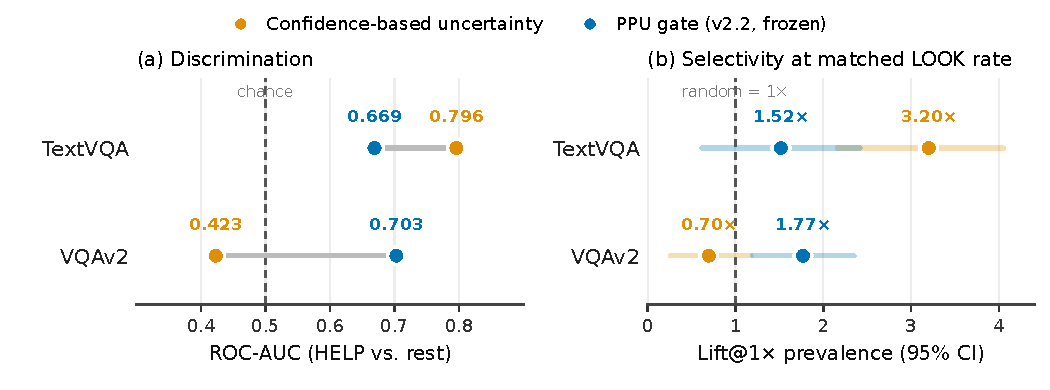
\includegraphics[width=\textwidth]{figures/fig1_confidence_reversal.pdf}
  \caption{
  \textbf{Answer confidence is not a stable proxy for perceptual need.}
  (a) Confidence-based uncertainty strongly discriminates \textsc{Help} states
  on TextVQA but falls below chance on VQAv2, while the frozen PPU gate remains
  above chance in both regimes.
  (b) At a prevalence-matched \textsc{Look} rate, confidence is highly selective
  on TextVQA but falls below random selection on VQAv2; PPU shows the
  complementary pattern. Horizontal intervals denote 95\% confidence intervals,
  and the dashed line denotes random ranking ($1\times$).
  }
  \label{fig:confidence-reversal}
\end{figure*}

% Fig. 2 — RQ4, near the fixed-budget paragraph
\begin{figure}[t]
  \centering
  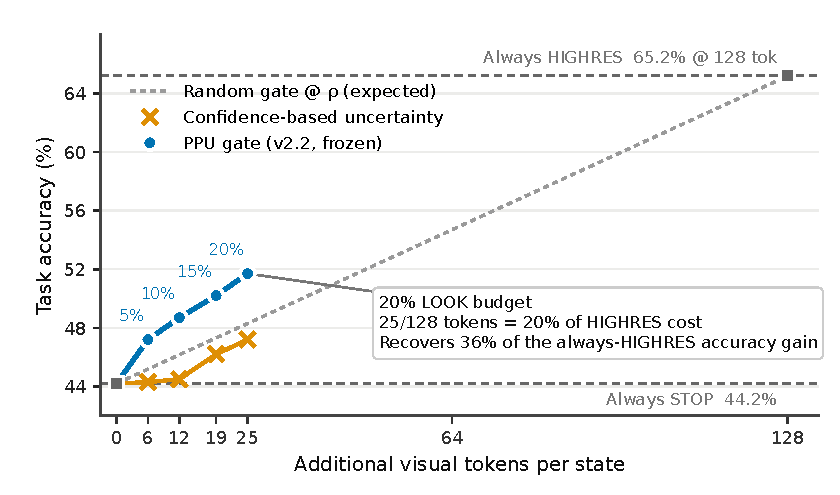
\includegraphics[width=\columnwidth]{figures/fig2_pareto_vqav2.pdf}
  \caption{
  \textbf{Accuracy--perception cost trade-off on VQAv2.}
  The frozen PPU gate consistently outperforms confidence-based selection at
  matched \textsc{Look} budgets. At a 20\% \textsc{Look} rate, PPU uses
  25 additional visual tokens per state, approximately 20\% of the
  always-\textsc{HighRes} cost, while recovering 36\% of the corresponding
  accuracy gain over always-\textsc{Stop}. The dashed horizontal lines denote
  the always-\textsc{Stop} and always-\textsc{HighRes} endpoints. The dotted
  grey line is the analytic expectation of a random gate that issues
  \textsc{Look} with probability $\rho$ independently of the state,
  $\mathrm{Acc}(\rho) = (1-\rho)\,\mathrm{Acc}_{\textsc{Stop}} + \rho\,\mathrm{Acc}_{\textsc{HighRes}}$,
  i.e.\ linear interpolation between the two endpoints; it is not an
  empirical average over sampled random gates.
  }
  \label{fig:pareto-vqav2}
\end{figure}

% ===================== REVISED (2026-08-22, v2) =====================
% Fig. 1 — headline, single column
\begin{figure}[t]
  \centering
  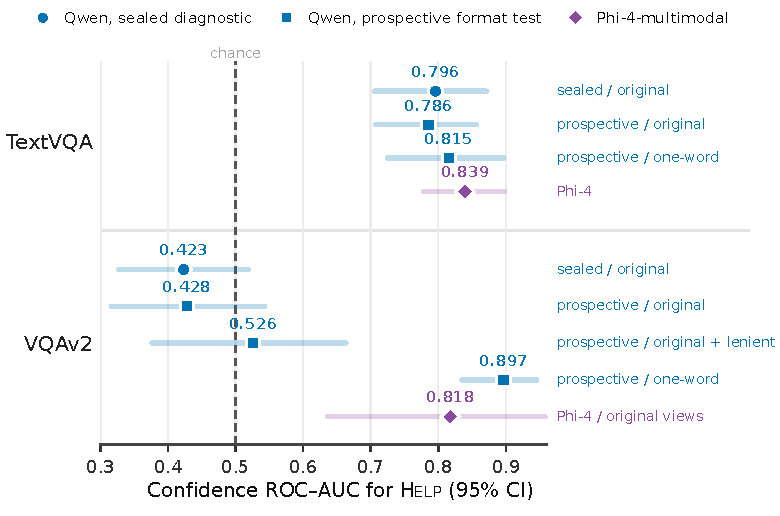
\includegraphics[width=\columnwidth]{figures/fig1_format_control.pdf}
  \caption{
  \textbf{Confidence--utility robustness across readers, prompts, and evaluation
  conditions.}
  Values are ROC--AUC of confidence-based uncertainty for ranking
  replicate-consistent \textsc{Help} states. On TextVQA, confidence remains
  strongly predictive of \textsc{Help} across the sealed lockbox, fresh
  prospective states, answer-format control, and Phi-4. On VQAv2, the
  below-chance Qwen pattern reproduces on fresh states under the original
  prompt, is only partially corrected by lenient rescoring, and shifts strongly
  above chance under one-word answer control. Horizontal bars show 95\%
  bootstrap confidence intervals; the dashed line denotes chance ROC--AUC.
  Unless marked lenient, points use strict scoring; Phi-4 views are
  Qwen-token-equivalent (TextVQA 192$\to$512; VQAv2 16$\to$192 for Phi-4,
  64$\to$192 for Qwen).
  }
  \label{fig:format-control}
\end{figure}

% Fig. 2 — single column, vertical 2-panel
\begin{figure}[t]
  \centering
  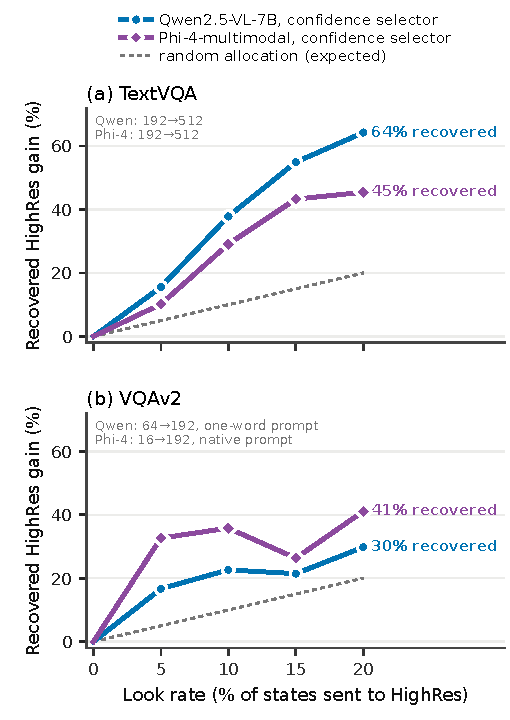
\includegraphics[width=\columnwidth]{figures/fig2_recovered_gain.pdf}
  \caption{
  \textbf{Confidence-based selection recovers a substantial share of the
  available perception gain at small \textsc{Look} budgets.}
  The $\rho$ least-confident states are sent to \textsc{HighRes} and the rest
  \textsc{Stop}; the $y$-axis is the recovered share of the always-\textsc{HighRes}
  gain, $(A_{\text{sel}}-A_{\textsc{Stop}})/(A_{\textsc{HighRes}}-A_{\textsc{Stop}})$,
  over the full lockbox population (replay-ambiguous states included), which
  removes backbone accuracy and coarse-budget differences. Random allocation
  recovers $\rho$ in expectation (dotted). (b) uses the one-word answer prompt
  for Qwen (64$\rightarrow$192) and Phi-4's native prompt with a 16-token coarse
  view (16$\rightarrow$192). Absolute accuracies are given in
  Fig.~\ref{fig:lookrate-abs}.
  }
  \label{fig:recovered-gain}
\end{figure}

% Supplementary — full width
\begin{figure*}[t]
  \centering
  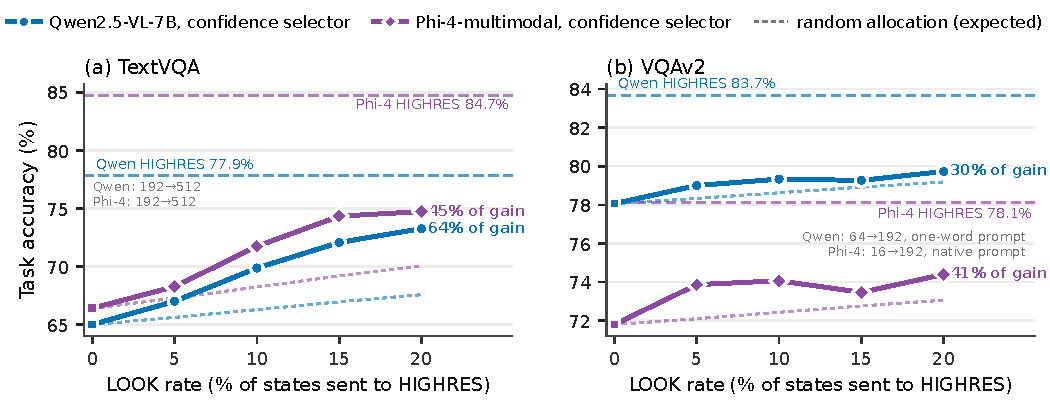
\includegraphics[width=\textwidth]{figures/figS_lookrate_abs.pdf}
  \caption{
  \textbf{Absolute accuracy vs.\ \textsc{Look} rate} for the confidence
  selector (solid), random allocation (dotted, expectation
  $(1-\rho)A_{\textsc{Stop}}+\rho A_{\textsc{HighRes}}$) and always-\textsc{HighRes}
  (dashed), full lockbox population. Curves for the two backbones are not
  directly comparable in level: they differ in base accuracy and, in (b), in
  coarse budget (Qwen 64$\rightarrow$192 with a one-word prompt; Phi-4
  16$\rightarrow$192, native prompt). Labels give the recovered share of the
  \textsc{HighRes} gain at a 20\% \textsc{Look} rate.
  }
  \label{fig:lookrate-abs}
\end{figure*}
